\begin{apendicesenv}

\partapendices

\chapter{PROTOCOLOS DE COMUNICAÇÃO}

A comunicação envolve a troca de uma série de mensagens entre duas entidades. Parte
fundamental para a comunicação bem sucedida é a premissa a respeito das informações
transmitidas e recebidas, como por exemplo a linguagem e o meio de transmissão
\cite{comer2000}. Caso as entidades envolvidas na comunicação não concordem em
relação a estas premissas, não será possível estabelecer um diálogo adequada.

Restrições a respeito do formato, meios de transmissão, e ações a serem tomadas no
envio e recebimento de mensagens são definidas por meio de protocolos. A partir do
momento em que duas entidades sigam o mesmo protocolo, pode-se garantir que a
comunicação será estabelecida. Assim como qualquer outra entidade, componentes de
\textit{hardware} e \textit{software} também estão sujeitos a protocolos de
comunicação \cite{kurose2012}.

Antes de abordar os protocolos de federação, é necessário entender a necessidade de
protocolos de comunicação a partir da utilização em redes de computadores. Também se
faz necessário discutir o processo de padronização desses protocolos, o que deve
ajudar na discussão a respeito da definição e utilização de padrões na construção de
sistemas federados.



\section{SUÍTES DE PROTOCOLOS}

No contexto da computação, redes de comunicação são construídas com diferentes
tecnologias de acordo com necessidades e restrições específicas, o que prejudica a
capacidade de intercomunicação entre dispositivos \cite{comer2000}. A Internet, por
exemplo, é uma coleção de redes menores que eventualmente utilizam tecnologias
diferentes, como é o caso de linhas telefônicas, e transmissão a rádio
\cite{tanenbaum2010}. Um desafio diferente é alcançar a intercomunicação em um
sistema complexo como tal, onde as redes que o compõem utilizam seus próprios
protocolos, desta vez específicos ao meio de transmissão.

De acordo com \cite{comer2000}, existem duas observações fundamentais ao projeto de
redes de comunicação:

\begin{enumerate}
  \item{Não existe nenhuma tecnologia de rede capaz de satisfazer às restrições de
        todos os possíveis contextos;}
  \item{Usuários desejam intercomunicação universal.}
\end{enumerate}

A primeira observação sugere que a necessidade de interoperabilidade eventualmente
pode surgir entre sistemas incompatíveis. Ainda assim, a discrepância deve ser
invisível ao usuário, que de qualquer forma espera a interoperabilidade, ponto
reafirmado pela segunda observação.

Esse tipo de interoperabilidade pode ser implementada tanto no nível das aplicações
quanto no nível da rede. Enquanto a primeira estratégia supõe que as aplicações
prevejam explicitamente suporte a cada uma das tecnologias, a segunda estratégia
é mapeada desde o \textit{hardware}, providenciando uma camada de abstração para os
componentes utilitários.

A intercomunicação no nível de rede (ou simplesmente internet \cite{comer2000})
também pode empregar um modelo de camadas. Neste caso, os protocolos são organizados
em uma hierarquia vertical, de acordo com seus objetivos. A interface entre cada
camada é bem definida, o que concede modularidade ao sistema \cite{kurose2012}.

Neste tipo de hierarquia as mensagens são enviadas sucessivamente da camada mais
superior até a camada mais inferior durante a transmissão, o inverso do que acontece
no recebimento. Apenas as camadas mais inferiores do transmissor e destinatário são
conectadas por meio de um meio de transmissão arbitrário, o que garante abstração do
meio para as camadas superiores.

\begin{figure}[h]
	\centering
		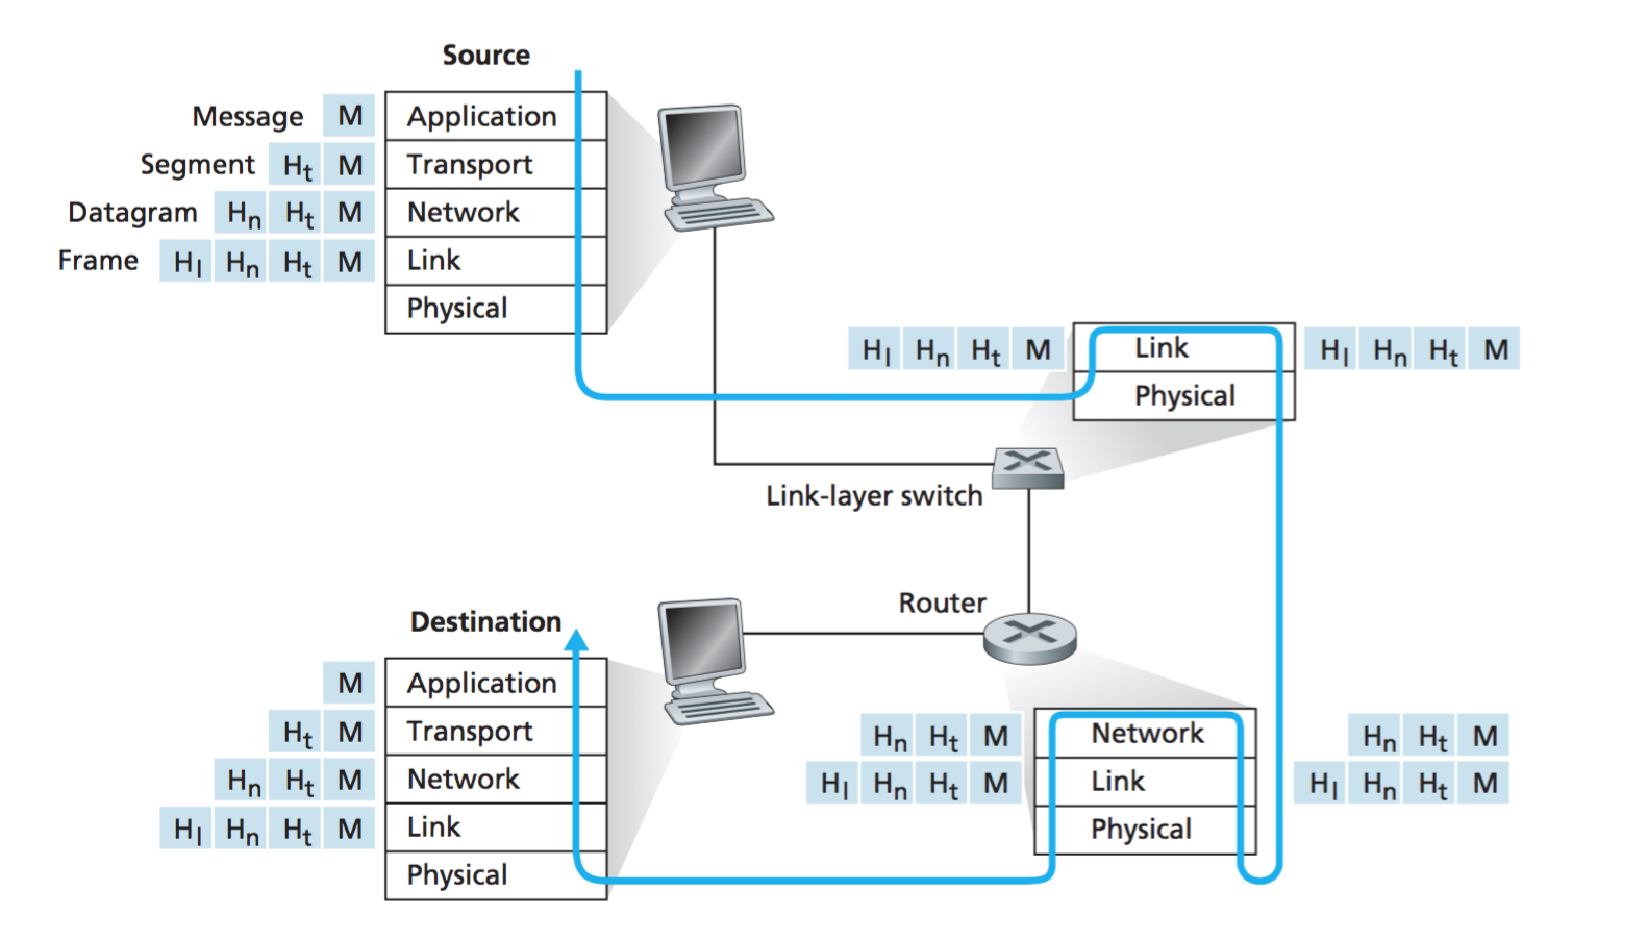
\includegraphics[keepaspectratio=true,scale=0.6]{figuras/encapsulamento.eps}
	\caption[Encapsulamento de mensagens entre camadas \cite{kurose2012}.]
          {Encapsulamento de mensagens em um modelo de camadas \cite{kurose2012}.}
	\label{fig:encapsulamento}
\end{figure}

A Figura \ref{fig:encapsulamento} mostra este processo no contexto do TCP/IP, também
conhecido como a suíte de protocolos da Internet. Neste caso, os protocolos de cada
camada adicionam um cabeçalho às mensagens recebidas do nível anterior, o que
permite a adição de informações adicionais destinadas ao mesmo protocolo
implementado no comunicante.



\section{PADRONIZAÇÃO DE PROTOCOLOS}

A definição de protocolos é apenas o primeiro passo para a intercomunicação de
sistemas. Se não existir um acordo a respeito da especificação utilizada será mais
difícil estabelecer a comunicação entre serviços \cite{kurose2012}. A padronização
garante o estabelecimento deste acordo.

\begin{sloppypar}
O conceito de efeito de rede indica que a adoção de um protocolo se torna mais
valiosa à medida que um maior número de entidades também o utilize
\cite{liebowitz1998}. Justifica-se portanto o interesse em incentivar a padronização
de protocolos.
\end{sloppypar}

A partir do momento em que uma série de entidades entra em consenso a respeito da
especificação de um protocolo, estabelece-se um padrão \textit{de facto}. A
iniciativa de padronização também pode surgir através de entidades regulamentadoras,
como a Organização Internacional para a Padronização (ISO), ou a \textit{Internet
Engineering Task Force} (IETF), o que leva ao estabelecimento padrões \textit{de
jure} \cite{tanenbaum2010}.

O processo de definição de novos padrões \textit{de jure} depende da entidade
regulamentadora relacionada, e ocasionalmente parte de padrões \textit{de facto} já
utilizados na comunidade. Geralmente uma especificação é proposta, discutida, e
revisada pela entidade antes de se tornar um padrão, o que no caso da ISO pode levar
de seis meses a alguns anos \cite{tanenbaum2010}.

Propostas e padrões estabelecidos devem ser documentados de alguma forma. A IETF
adota o formato de \textit{Request for Comments} (RFC), publicações que descrevem
completamente uma especificação, e estão disponíveis a consulta pela comunidade.

Uma proposta deve cumprir uma série de requisitos antes de ser endossado por uma
organização. No caso da IETF, cada proposta passa por vários níveis de maturidade
até alcançar a categoria de padrão. Cada um destes níveis pode ser alcançado ao
satisfazer as recomendações de determinados grupo da comunidade. Um exemplo destes
requisitos é a exigência de uma prova de conceito de interoperabilidade, como uma
implementação de referência entre duas ou mais entidades distintas \cite{rfc1280}.

Protocolos de federação também estão sujeitos ao efeito de rede, e apresentam as
mesmas necessidades de padronização. O \textit{Simple Mail Transfer Protocol} é um
exemplo de especificação utilizado na interoperabilidade de sistemas federados que
passou por um esforço oficial de padronização, tornando-se um caso interessante na
análise deste processo.


\subsection{Simple Mail Transfer Protocol}

\begin{sloppypar}
Um sistema de \textit{e-mails} pode ser considerado federado, já que respeita a
definição de implementações interoperáveis no modelo cliente servidor apresentada
por \cite{barocas2012}. O SMTP é um dos protocolos utilizados na implementação de
interoperabilidade entre serviços distintos.
\end{sloppypar}

Trata-se de um protocolo para o transporte e entrega de mensagens de e-mail entre
processos. A especificação garante que a troca de mensagens aconteça entre clientes
que se localizam em redes diferentes, o que permite a construção de um serviço que
funcione de maneira confiável sobre a internet \cite{rfc2821}.

Caracterizado como um protocolo orientado a conexões entre clientes e servidores, ou
transmissores e receptores, o SMTP é guiado por uma série de comandos predefinidos.
Os servidores também são responsáveis por retransmitir mensagens, caso não sejam os
destinatários finais \cite{kurose2012}.

A troca de mensagens geralmente acontece em um único salto após o estabelecimento de
uma conexão orientada entre o remetente e o destinatário. A retransmissão de
mensagens é uma alternativa, utilizada por exemplo em casos em que um usuário moveu
sua caixa de e-mails de um servidor para outro e deseja receber as mensagens no seu
novo endereço.

\begin{figure}[h]
	\centering
		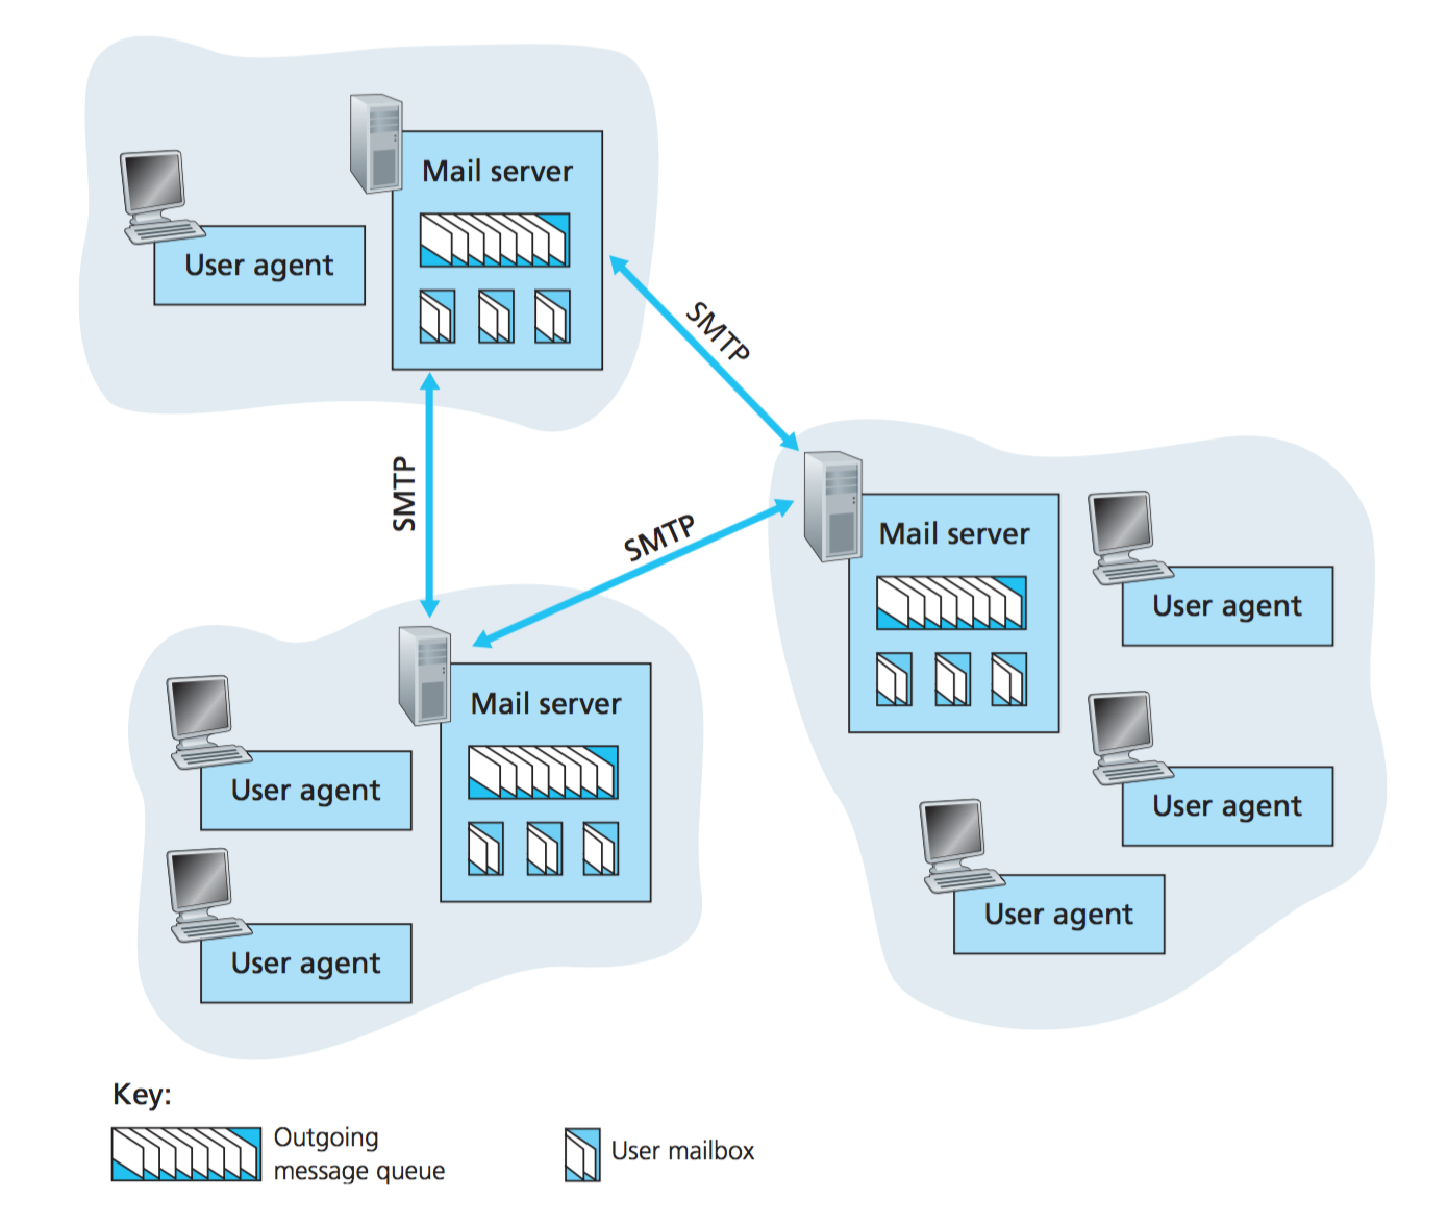
\includegraphics[keepaspectratio=true,scale=0.6]{figuras/smtp_internet.eps}
	\caption{Uma visão geral de um sistema de e-mails \cite{kurose2012}.}
	\label{fig:smtpInternet}
\end{figure}

Como pode ser visto na Figura \ref{fig:smtpInternet}, o SMTP é um protocolo
intermediário entre servidores de e-mail que alternam entre os papéis de transmissor
e receptor. Cada um destes servidores possui seus próprios clientes, constituindo
sistemas menores onde a interação não é necessariamente coberta pela especificação
do SMTP. Os mecanismos de comunicação entre o servidor e o usuário destes sistemas
não é necessariamente compatível e eventualmente utilizam outros padrões, como por
exemplo POP3 ou IMAP \cite{tanenbaum2010}.

O SMTP eventualmente passou pelo processo de padronização da IETF que levou à
publicação de uma RFC. Trata-se de um padrão \textit{de jure} aberto, definido por
uma organização ainda que adotado pelo mercado.

Considerando a descentralização da arquitetura e a padronização do protocolo,
qualquer novo sistema é capaz de implementar e se tornar parte da federação com
relativa facilidade. Nestes casos a heterogeneidade entre os sistemas intermediários
é completamente transparente para os usuários do serviço, o que o indica como um
protocolo de federação bem sucedido.

\chapter{SUPORTE À FEDERAÇÃO}

Já existe uma iniciativa de federação no Noosfero em desenvolvimento por parte da
comunidade \footnote{A discussão a respeito da federação no Noosfero está registrada
no endereço a seguir
\url{https://softwarepublico.gov.br/gitlab/noosferogov/noosfero/wikis/federacao}.},
tendo o autor deste trabalho colaborado desde então. O objetivo é possibilitar a
integração tanto com outras instâncias do Noosfero como com outras redes sociais, o
que exige a adoção de especificações que tenham o mínimo de aderência na comunidade.
A utilização de padrões difundidos amplia as possibilidades de integração dentre
outras redes sociais federadas.

Antes da execução deste trabalho, os protocolos Diaspora e OStatus já haviam sido
escolhidos como referência para a implementação da federação no Noosfero, resultado
de uma observação das discussões e execução de projetos como o Hubzilla, Friendica e
o próprio Diaspora.

As primeiras contribuições com a federação no Noosfero tiveram início antes deste
trabalho, e estão descritas na Subseção \ref{subsec:federacao_noosfero}. Os
resultados relativos à integração com outras redes, apresentados na Subseção
\ref{subsec:federacao_externa}, são produtos deste projeto.


\section{Federação entre redes Noosfero}
\label{subsec:federacao_noosfero}

As atividades de implementação de federação já desenvolvidas podem ser separadas em
quatro fases, que cumpriram objetivos distintos de integração, que cobrem desde as
funcionalidades até a reestruturação da arquitetura da aplicação.

Foi definido que um usuário de uma rede Noosfero pode acessar qualquer outra
instância com as credenciais de sua rede de origem. Um usuário federado deve ser
capaz de visualizar conteúdos públicos, comentar publicações, seguir usuários, e
deixar mensagens em murais. As notificações destas interações devem ser entregues
tanto aos usuários na rede local, quanto ao usuário na rede de origem.

O protocolo construído entre redes Noosfero é baseado nas especificações do
WebFinger e OAuth para a descoberta de identidade e autorização de perfis,
respectivamente. Em relação à comunicação entre as redes, o protocolo Diaspora foi
definido como referência.

\subsection{Fase 1: preparação}

Até a versão 1.5 do Noosfero, todos os relacionamentos entre as entidades da rede
eram baseados no conceito de relacionamento simétrico. No entanto, as demais redes
federadas, e a maioria dos padrões mais implementados, trabalham apenas com o
conceito de relacionamentos assimétricos, o que incentivou o desenvolvimento da
funcionalidade de seguidores no Noosfero.

Na fase de preparação foram introduzidos os relacionamentos assimétricos através
desta funcionalidade. Os seguidores são notificados a respeito de atividades
públicas de perfis seguidos. No Noosfero, cada perfil pode permitir ou não que
usuários o sigam. Usuários por sua vez organizam os perfis seguidos em círculos,
categorizando suas relações.

\subsection{Fase 2: intercomunicações}

Durante a fase de intercomunicações foi construída a infraestrutura básica para a
integração entre redes Noosfero. Ambientes e usuários externos foram introduzidos à
arquitetura do Noosfero, que passa a suportar ações de usuários que não possuem
perfis locais.

O conceito de usuário externo introduzido nesta fase é importante para toda a
implementação da federação do Noosfero. Um usuário local do Noosfero é definido por
basicamente dois objetos de negócio --- um usuário, que armazena as credenciais de
acesso, e um perfil, que armazena suas demais informações na aplicação.

Um usuário externo não possui credenciais de acesso na instância visitada, apenas um
objeto que representa o seu perfil externo, e que do ponto de vista da implementação
deve ser capaz de reproduzir o comportamento de um perfil comum. A implementação
alcançada faz uso de métodos \textit{stub} e relações polimórficas para a reprodução
do comportamento.

Nesta fase também foi implementada a especificação do WebFinger, que já está sendo
utilizada para a descoberta de usuários na autenticação entre redes Noosfero.

Inicialmente, apenas as redes listadas no diretório central do Noosfero
\footnote{\url{directory.noosfero.org}} podem ser habilitadas no painel de
administração da federação. A descentralização desta lista ou a automatização do
processo de descoberta não fizeram parte do planejamento inicial.

\subsection{Fase 3: integração externa}

A fase de integração externa teve como objetivo aproveitar a infraestrutura de
usuários externos para autenticar usuários de outros serviços sem a necessidade de
perfis locais. Com isto, usuários de sistemas que suportem OAuth podem acessar o
Noosfero, consumir conteúdo, e executar um conjunto limitado de ações.

Durante esta etapa, o \textit{plugin} que torna o Noosfero em um cliente OAuth foi
evoluído para permitir que usuários possam tanto criar um perfil local a partir das
informações da rede de origem, como também apenas acessar o Noosfero com um perfil
temporário. Por enquanto, os únicos fornecedores OAuth suportados são o Google,
Facebook, Twitter, GitHub, e o próprio Noosfero. No entanto, novos fornecedores
podem ser facilmente adicionados.

\subsection{Fase 4: inter-relações}

A última fase de desenvolvimento da federação de redes Noosfero foi implementar o
relacionamento entre usuários de instâncias diferentes. De modo geral, esta fase
consistiu em permitir que usuários externos sejam capazes de seguir perfis, comentar
conteúdos, e publicar em murais de outros usuários.

De forma a permitir relações entre usuários federados foi necessário refatorar a
funcionalidade de seguidores, adicionando o suporte a perfis externos. Neste ponto,
usuários federados podem tanto seguir usuários locais, quanto serem seguidos por
eles.

Essa fase também envolve a implementação da infraestrutura de troca de mensagens,
que seria utilizada nas notificações e interações entre os usuários. Até a
execução deste trabalho esse mecanismo não foi completamente definido.

\chapter{IMPLEMENTAÇÃO}

A documentação da biblioteca utilizada para a implementação do protocolo não cobre
todos os aspectos da especificação, portanto foi necessário instanciar dois
\textit{pods} locais do Diaspora para analisar a comunicação. A comunicação do
Diaspora depende que cada um dos \textit{pods} responda a HTTPS e seja capaz de
resolver os nomes dos demais servidores.

Para os testes desse trabalho foram utilizadas duas máquinas virtuais com Debian 8
em rede privada, com os nomes registrados no arquivo de \textit{hosts} para a
resolução local. Em cada uma das máquinas, o Diaspora foi servido por um servidor
NGINX com SSL configurado com um certificado auto-assinado. Para que a comunicação
não fosse prejudicada pela verificação dos certificados, eles foram manualmente
adicionados aos certificados reconhecidos em cada uma das máquinas.

\section{AUTENTICAÇÃO COM O DIASPORA}

A federação através do Diaspora foi planejada com base na implementação já existente
no Noosfero, que conta com um mecanismo de autenticação entre as redes. Por esse
motivo inicialmente se julgou necessário permitir a autenticação de usuários com
credenciais de redes Diaspora.

O Diaspora não disponibiliza nenhum \textit{endpoint} de \textit{login} em sua API,
mas implementa o papel de fornecedor de identidades OpenID Connect\footnote{O OpenID
Connect é um padrão de autenticação construído sobre a segunda versão do OAuth.
\url{http://openid.net/specs/openid-connect-core-1_0.html}}. Portanto, a fim de
utilizar as credenciais do Diaspora, é necessário que o Noosfero possa desempenhar o
papel de cliente OpenID.

Mesmo que o Noosfero também forneça identidades OpenID, ainda não seria possível
usar credenciais locais para a autenticação em \textit{pods} Diaspora, que utiliza
apenas estratégias de autenticação local. Isso reforçou a decisão de implementar
apenas a função de cliente OpenID por enquanto.

Ainda que o \textit{plugi-in} tenha sido implementado como parte deste trabalho, o
restante da federação não depende deste mecanismo de autenticação, já que os
usuários só interagem com o servidor remoto através de sua rede de origem.

\subsection{Desenvolvimento do plugin OpenID Client}

Apesar do Noosfero já oferecer suporte à autorização com OAuth 1.0 através de um
\textit{plugin}, foi necessário implementar o suporte ao OpenID. A decisão foi criar
um novo \textit{plugin} que transforme o Noosfero em um cliente OpenID.

A \textit{gem} openid\char`_connect foi utilizada na implementação do consumidor. A
biblioteca já oferece as diretrizes de descoberta, registro de clientes e
autenticação, todas interações que envolvem requisições HTTP ao servidor fornecedor.
Um perfil externo também é criado no Noosfero para armazenar algumas informações do
perfil remoto, como \textit{link} para o seu perfil, ou sua imagem do avatar.

Os passos realizados pelo \textit{plugin} na autenticação de um usuários são:

\begin{enumerate}
  \item{O usuário digita o endereço do fornecedor OpenID de sua escolha;}
  \item{O Noosfero tenta descobrir informações a respeito do provedor, solicitando
        informações do emissor de identidades;}
  \item{Caso a resposta do provedor seja válida, o Noosfero solicita o registro como
        um novo cliente, solicitando acesso a informações necessárias para a criação
        de um perfil externo;}
  \item{A requisição é redirecionada ao fornecedor OpenID, onde o usuário deve se
        autenticar, e revisar a solicitação enviada pelo Noosfero;}
  \item{Se o usuário se autenticar no seu provedor e aprovar as informações
        solicitadas, a resposta do servidor será usada na criação de um perfil
        externo, e o usuário será autenticado no Noosfero}
\end{enumerate}

\end{apendicesenv}
